%%%%%%%%%%%%%%%%%%%%%%%%%%%%%%%%%%%%%%%%%%%%%%%%%%%%%%%%%%%%%%%%%%%%%%%%%%%%%%%%%%%%%%%%%%%%%%%%%%%%%%%%%%%%%%%%%%%%%%%%%%%%%
%Configurations
%%%%%%%%%%%%%%%%%%%%%%%%%%%%%%%%%%%%%%%%%%%%%%%%%%%%%%%%%%%%%%%%%%%%%%%%%%%%%%%%%%%%%%%%%%%%%%%%%%%%%%%%%%%%%%%%%%%%%%%%%%%%%
\documentclass[12pt,ignorenonframetext,aspectratio=1610]{beamer}

\mode<presentation> {
  \usetheme{Berkeley}
  \setbeamercovered{transparent}
  \usecolortheme{dolphin}
  \usefonttheme{structuresmallcapsserif}
  \useoutertheme{infolines} 
  \definecolor{forestgreen(web)}{rgb}{0.13, 0.55, 0.13}
	}

%\usetheme{Copenhagen}
%\usecolortheme{dolphin}
%\usefonttheme{structuresmallcapsserif}
%\useoutertheme{infolines} %adiciona as notas de rodapé dos slides
%\setbeamercovered{transparent}
%\setbeamertemplate{navigation symbols}{} %Quando ativo esta opção os símbolos de navegação desaparecem
%\beamertemplatetransparentcoveredhigh
%\useinnertheme{circles}
%\definecolor{forestgreen(web)}{rgb}{0.13, 0.55, 0.13}
%\bibliographystyle{plain}

%%%%%%%%%%%%%%%%%%%%%%%%%%%%%%%%%%%%%%%%%%%%%%%%%%%%%%%%%%%%%%%%%%%%%%%%%%%%%%%%%%%%%%%%%%%%%%%%%%%%%%%%%%%%%%%%%%%%%%%%%%%%%
%Packages
%%%%%%%%%%%%%%%%%%%%%%%%%%%%%%%%%%%%%%%%%%%%%%%%%%%%%%%%%%%%%%%%%%%%%%%%%%%%%%%%%%%%%%%%%%%%%%%%%%%%%%%%%%%%%%%%%%%%%%%%%%%%%
\usepackage[portuguese]{babel} % Traduz para o Português do Brasil
\usepackage[utf8]{inputenc} % Reconhece acentuação
\usepackage{ragged2e} % Mais opções de alinhamento
\usepackage[rightcaption]{sidecap}
\usepackage{graphicx} %Para melhor ajuste da posição de figuras
\usepackage{tikz} %Inserir figuras feitas com tikz
\usepackage{subfig} %Inserir subfiguras
\usepackage{multicol}
\usepackage[alf,abnt-emphasize=bf]{abntex2cite}
\usepackage{filecontents}
\usepackage{tikz}
\usetikzlibrary{mindmap,trees}
\usepackage{amsmath}
\usepackage{booktabs}
\usepackage{lscape}
\usepackage{pdflscape}
\usepackage{algorithmic}
\usepackage[font=small,labelfont=bf]{caption}
\usepackage{wrapfig}
\usepackage{xcolor}
\usepackage[autostyle]{csquotes}
\usepackage{tikzsymbols}

%Algoritmo
\usepackage[portugues,ruled,lined]{algorithm2e}
\usepackage{caption}
\makeatletter
\newcommand{\RemoveAlgoNumber}{\renewcommand{\fnum@algocf}{\AlCapSty{\AlCapFnt\algorithmcfname}}}
\newcommand{\RevertAlgoNumber}{\algocf@resetfnum}
\makeatother
\usepackage{listings}
\renewcommand{\baselinestretch}{1}
\SetAlFnt{\normalsize}

%%%%%%%%%%%%%%%%%%%
\usepackage[framemethod=TikZ]{mdframed}
\mdfdefinestyle{MyFrame}{%
	linecolor=blue,
	outerlinewidth=.5pt,
	roundcorner=25pt,
	innertopmargin=\baselineskip,
	innerbottommargin=\baselineskip,
	innerrightmargin=50pt,
	innerleftmargin=2pt,
	backgroundcolor=gray!5!white,
	}

\newmdenv[linecolor=black,leftmargin=1em,rightmargin=1em,innertopmargin=1em,innerbottommargin=1em]{infobox}
%\bibliographystyle{abntex2-alf}
%\bibliographystyle{plain}
%\bibliographystyle{alpha}

%\pgfdeclareimage[height=1cm, width=2cm]{rbras63}{rbras63}
%\logo{\pgfuseimage{rbras63}}
%\setbeamertemplate{footline}[frame number]
	
%%%%%%%%%%%%%%%%%%%%%%%%%%%%%%%%%%%%%%%%%%%%%%%%%%%%%%%%%%%%%%%%%%%%%%%%%%%%%%%%%%%%%%%%%%%%%%%%%%%
%Preamble
%%%%%%%%%%%%%%%%%%%%%%%%%%%%%%%%%%%%%%%%%%%%%%%%%%%%%%%%%%%%%%%%%%%%%%%%%%%%%%%%%%%%%%%%%%%%%%%%%%%
\title[Machine Learning e Biometria Florestal]{{\normalsize O vizinho mais próximo ponderado na predição da biomassa da parte aérea de árvores em florestas tropicais}}

\author[Deivison V. Souza]{\textbf{Deivison Venicio Souza\inst{}}}

\institute[]
{\inst{}%
	\scriptsize Universidade Federal Pará - UFPA \\ 
	\scriptsize Engenheiro Florestal, Me. Ciências Florestais \\ 
	\scriptsize Programa de Pós-graduação em Engenharia Florestal - UFPR \\
	\href{mailto:deivisonvs@ufpa.br}{\scriptsize (deivisonvs@ufpa.br)}
	}

\date[\today]{\footnotesize \textbf{63ª Reunião Anual da Região Brasileira da Sociedade Internacional de Biometria (RBras)}}

\titlegraphic{\begin{columns}
		\begin{column}{0.3\textwidth}
			\begin{figure}%
				
\includegraphics[height=1cm, width=2cm]{Fig/biofix.jpg}%
			\end{figure}
		\end{column}
		\begin{column}{0.3\textwidth}
			\begin{figure}%
				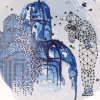
\includegraphics[height=1cm, width=1.5cm]{Fig/rbras63.png}%
			\end{figure}
		\end{column}\end{columns}}

%\author[Deivison Souza (UFPA)]{\textbf{Deivison Venicio Souza} \\ \scriptsize Doutorando do Programa de Pós-graduação em Engenharia Florestal - UFPR \\ Linha de Pesquisa: Manejo Florestal \\ %(deivisonvs@ufpa.br)}

%\institute[UFPA]{\textbf{Universidade Federal do Pará}}

%\date[\today]{\scriptsize Curitiba, PR \\ \today}

%\titlegraphic{\includegraphics[scale=0.18]{ilogo.png}}
%\logo{\includegraphics[height=1.5cm]{ilogo.png}}

%%%%%%%%%%%%%%%%%%%%%%%%%%%%%%%%%%%%%%%%%%%%%%%%%%%%%%%%%%%%%%%%%%%%%%%%%%%%%%%%%%%%%%%%%%%%%%%%%%%
% BEGINNING OF THE DOCUMENT
%%%%%%%%%%%%%%%%%%%%%%%%%%%%%%%%%%%%%%%%%%%%%%%%%%%%%%%%%%%%%%%%%%%%%%%%%%%%%%%%%%%%%%%%%%%%%%%%%%%
\begin{document}

\begin{frame}
 \titlepage
\end{frame}

%%%%%%%%%%%%%%%%%%%%%%%%%%%%%%%%%%%%%%%%%%%%%%%%%%%%%%%%%%%%%%%%%%%%%%%%%%%%%%%%%%%%%%%%%%%%%%%%%%%
% TABLE OF CONTENTS
%%%%%%%%%%%%%%%%%%%%%%%%%%%%%%%%%%%%%%%%%%%%%%%%%%%%%%%%%%%%%%%%%%%%%%%%%%%%%%%%%%%%%%%%%%%%%%%%%%%

\begin{frame}
\frametitle{Conteúdo}
\tableofcontents
\end{frame}

%%%%%%%%%%%%%%%%%%%%%%%%%%%%%%%%%%%%%%%%%%%%%%%%%%%%%%%%%%%%%%%%%%%%%%%%%%%%%%%%%%%%%%%%%%%%%%%%%%%
\begin{frame}[c]{}
	\transwipe
	\begin{center}
				
		``{\large Esta apresentação constitui uma pequena parte da pesquisa inédita de doutorado (em andamento) do palestrante que está sendo conduzida no Programa de Pós-graduação em Engenharia Florestal da UFPR.}"
				
	\end{center}
	
\end{frame}

%%%%%%%%%%%%%%%%%%%%%%%%%%%%%%%%%%%%%%%%%%%%%%%%%%%%%%%%%%%%%%%%%%%%%%%%%%%%%%%%%%%%%%%%%%%%%%%%%%%
\section{Biomassa}
\begin{frame}[c]{}
		\transwipe
		\justifying
		
		\textbf{O que é?} \newline
		
		O termo “biomassa” se refere à massa dos componentes de uma árvore excluindo-se a água, isto é, a “\textbf{massa seca}” da árvore (BATISTA et al., 2014). \newline
		
		
	    \textbf{Por que?} \newline
		
		 A biomassa precisa ser determinada e estimada de forma fidedigna. Do contrário não haverá consistência na \textbf{quantificação do carbono fixado nos ecossistemas florestais} (SANQUETTA, 2002).
	
\end{frame}

%%%%%%%%%%%%%%%%%%%%%%%%%%%%%%%%%%%%%%%%%%%%%%%%%%%%%%%%%%%%%%%%%%%%%%%%%%%%%%%%%%%%%%%%%%%%%%%%%%%
\begin{frame}[c]{}
		
		\textbf{Compartimentalização da biomassa de árvores}
		
	\begin{center}
		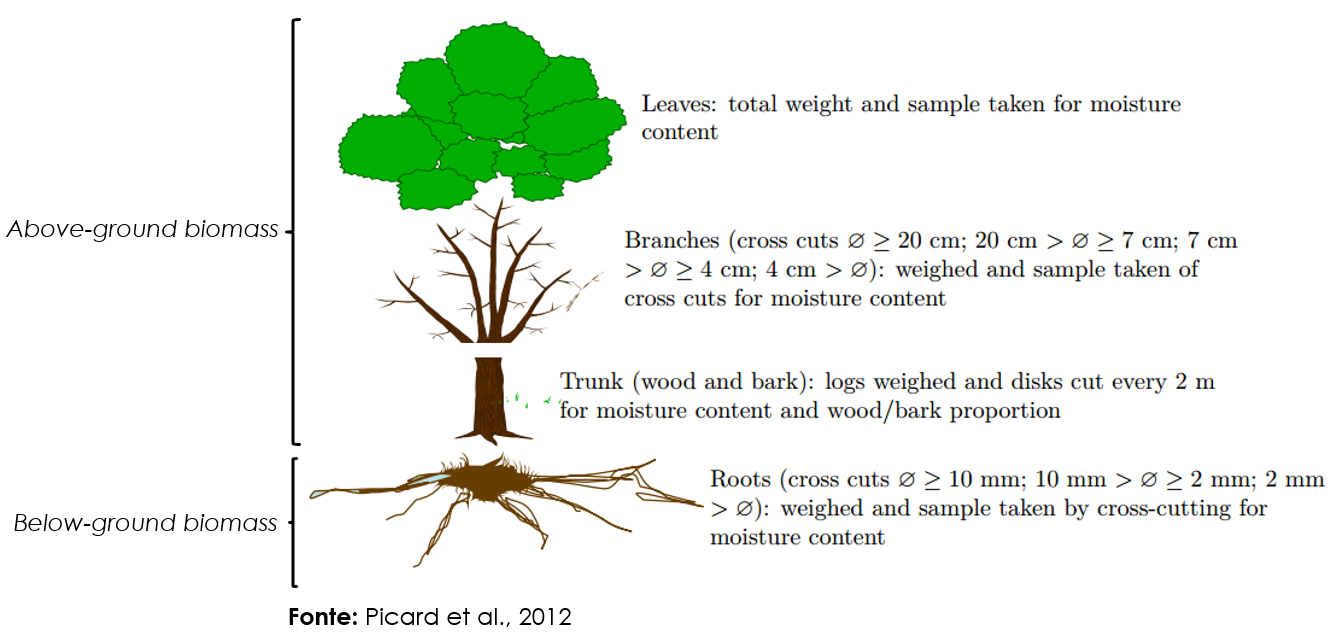
\includegraphics[scale=0.47]{Fig/Biomass3}
	\end{center}
	
\end{frame}

%%%%%%%%%%%%%%%%%%%%%%%%%%%%%%%%%%%%%%%%%%%%%%%%%%%%%%%%%%%%%%%%%%%%%%%%%%%%%%%%%%%%%%%%%%%%%%%%%%%
\begin{frame}[c]{}
		
		\textbf{Como quantificar a biomassa de árvores?}
			
	\begin{center}
		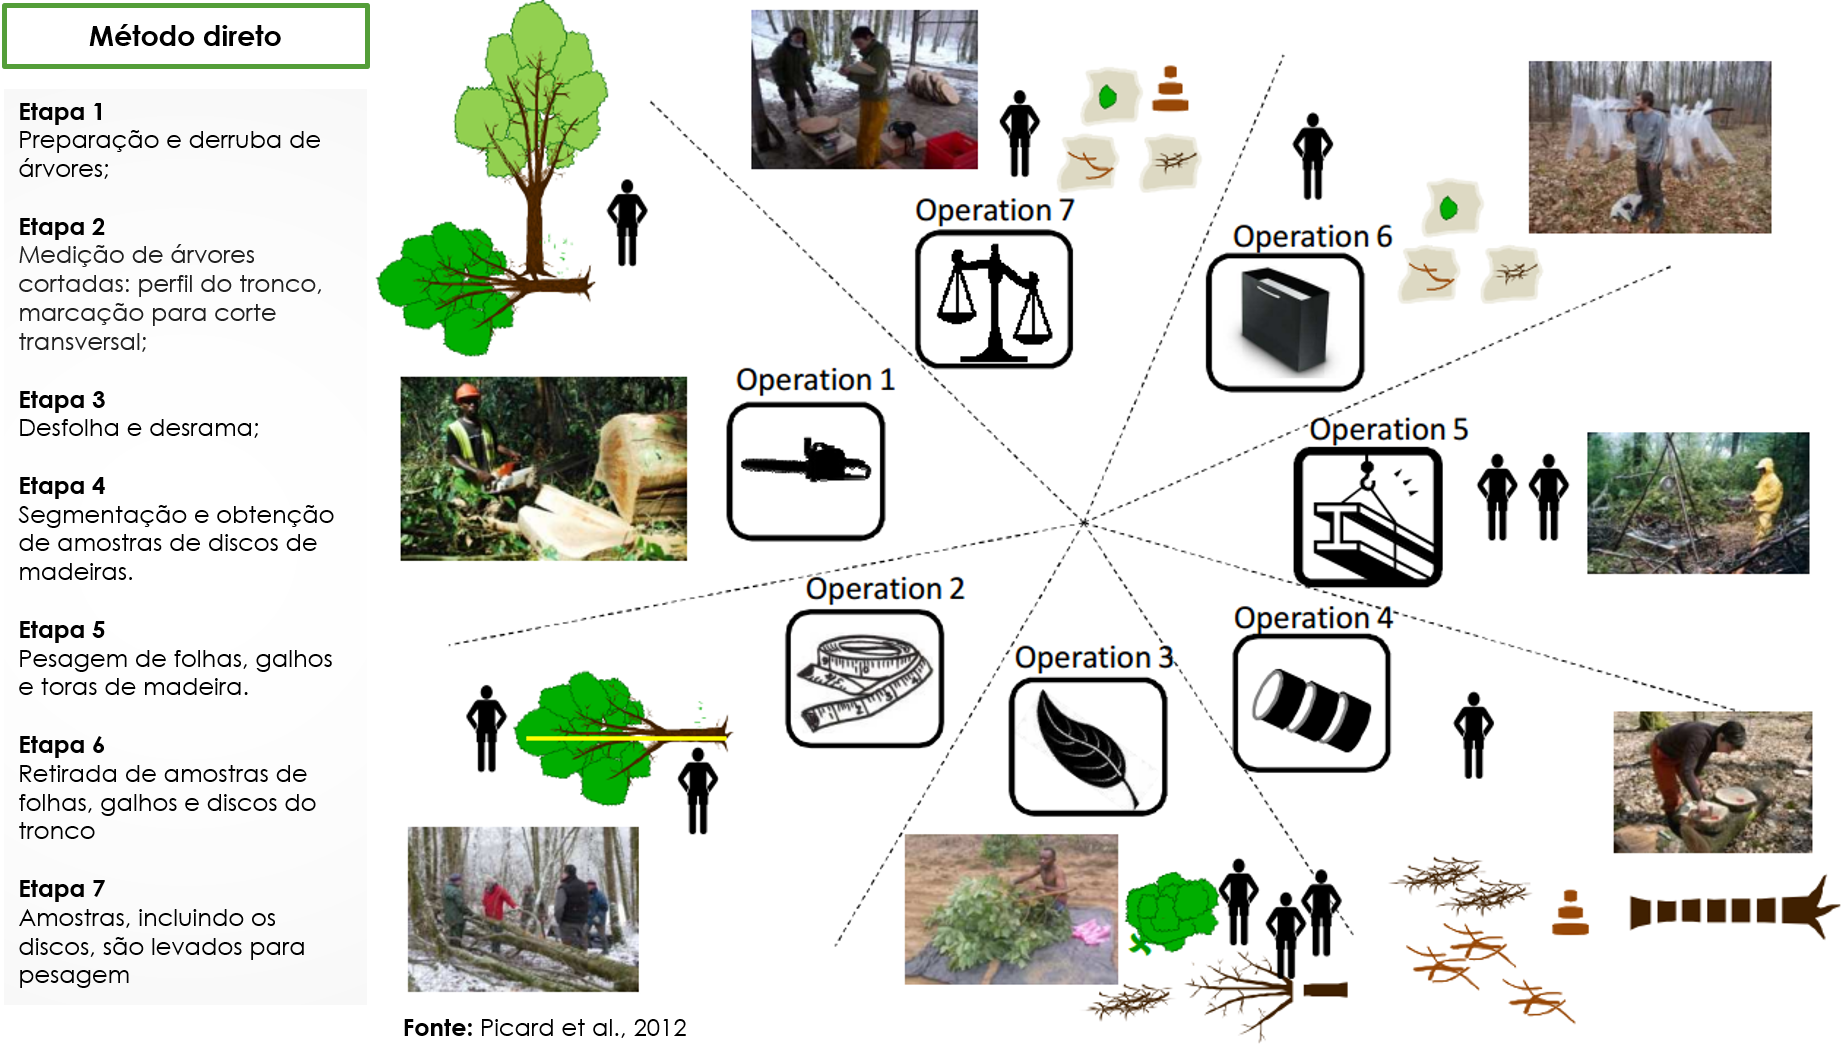
\includegraphics[scale=0.35]{Fig/Biomass2}
	\end{center}
	
\end{frame}

%%%%%%%%%%%%%%%%%%%%%%%%%%%%%%%%%%%%%%%%%%%%%%%%%%%%%%%%%%%%%%%%%%%%%%%%%%%%%%%%%%%%%%%%%%%%%%%%%%%
\begin{frame}[t]{}
	
	\textbf{PROBLEMA?} \newline
	
\textbf{Floresta Multiânea}: \newline

- Simplesmente impossível, impraticável!  \newline

- Portanto, é necessário aperfeiçoar os métodos indiretos de estimativa de biomassa florestal \cite{higuchi2004dinamica}. \newline

\textbf{Potencial frente à Regressão Tradicional:} \textcolor{blue}{\textbf{Aprendizagem de Máquina}}. \newline

\end{frame}

%%%%%%%%%%%%%%%%%%%%%%%%%%%%%%%%%%%%%%%%%%%%%%%%%%%%%%%%%%%%%%%%%%%%%%%%%%%%%%%%%%%%%%%%%%%%%%%
\begin{frame}[c]{Problemática}
	
	\transwipe
	\justifying
	
	\textbf{Problemas com uso da regressão... } \newline
	
	\begin{infobox}
			
1 - \textbf{Nem sempre se consegue obter modelos alométricos satisfatórios}, em termos de precisão das estimativas que, muitas vezes, resultam em níveis de erro para além limiares de tolerância nas medidas florestais \cite{sanquetta2013use}; \\

2 - \textbf{Grande variabilidade natural dos dados de biomassa}: $>$ variabilidade de biomassa $>$ diâmetro $\Longrightarrow$ Espécies nativas de regiões tropicais e subtropicais \cite{sanquetta2015comparison};
		
	\end{infobox}
	
\end{frame}

%%%%%%%%%%%%%%%%%%%%%%%%%%%%%%%%%%%%%%%%%%%%%%%%%%%%%%%%%%%%%%%%%%%%%%%%%%%%%%%%%%%%%%%%%%%%%%%%
\begin{frame}[c]{Problemática}
	
	\transwipe
	\justifying
	
	\textbf{Problemas com uso da regressão... } \newline
	
	\begin{infobox}
		
		\begin{center}
			\textbf{Problemática?} \\
		\end{center}
		
       3) \textbf{Formulação matemática única} $\Longrightarrow$ Pode não reproduzir a elevada variabilidade natural dos dados de biomassa. Afetar a qualidade do modelo e fornecer estimativas viesadas \cite{sanquetta2013use}; e \\

       4) \textbf{Atendimento a pressuposições da regressão} $\Longrightarrow$ aditividade e linearidade, independência dos resíduos, homocedasticidade e normalidade de resíduos, inexistência de multicolinearidade.
		
	\end{infobox}
	
\end{frame}

%%%%%%%%%%%%%%%%%%%%%%%%%%%%%%%%%%%%%%%%%%%%%%%%%%%%%%%%%%%%%%%%%%%%%%%%%%%%%%%%%%%%%%%%%%%%%%%%
\begin{frame}[c]{Problemática}
	
	\transwipe
	\justifying
	
	\textbf{Potencial: Aprendizagem de Máquina} \newline
	
	\begin{infobox}
		
		\begin{center}
			\textbf{Modelagem não-paramétrica} \\
		\end{center}
		
Estudos recentes têm despertado para o potencial da técnica de mineração de dados (\textbf{Data Mining}) na predição de variáveis biométricas. (ex.: \cite{sanquetta2013use, sanquetta2015comparison})
		
	\end{infobox} \quad
		
\end{frame}

%%%%%%%%%%%%%%%%%%%%%%%%%%%%%%%%%%%%%%%%%%%%%%%%%%%%%%%%%%%%%%%%%%%%%%%%%%%%%%%%%%%%%%%%%%%%%%%%
% OBJETIVO
%%%%%%%%%%%%%%%%%%%%%%%%%%%%%%%%%%%%%%%%%%%%%%%%%%%%%%%%%%%%%%%%%%%%%%%%%%%%%%%%%%%%%%%%%%%%%%%%

\section{Objetivo geral}
\begin{frame}[c]{Objetivo geral}
	\transwipe
	\begin{center}
		{\Large \textbf{OBJETIVO GERAL}}
	\end{center}
	
\end{frame}

%%%%%%%%%%%%%%%%%%%%%%%%%%%%%%%%%%%%%%%%%%%%%%%%%%%%%%%%%%%%%%%%%%%%%%%%%%%%%%%%%%%%%%%%%%%%%%%%%%%
\begin{frame}[c]{Objetivo geral}

\transwipe
\justifying

\textbf{Objetivo geral} \newline

O principal objetivo deste estudo foi aplicar uma abordagem não-paramétrica na estimativa da biomassa da parte aérea de árvores em florestas tropicais usando do algoritmo \textcolor{blue}{\textit{Weighted k}-Nearest-Neighbor (\textit{wk}NN)} implementado por \citeonline{R-kknn} na library "kknn" do ambiente estatístico R; e \newline

Prover uma comparação do desempenho preditivo do modelo \textit{wk}NN final (ajustado com todos dados e usando da configuração ótima de hiperparâmetros) frente ao \textcolor{blue}{Modelo Pantropical} proposto por Chave et al. (2014). \newline \newline


{\scriptsize Chave et al. (2014). Improved allometric models to estimate the aboveground biomass of tropical trees. \textbf{Global change biology}, 20(10), 3177-3190.}

\end{frame}

%%%%%%%%%%%%%%%%%%%%%%%%%%%%%%%%%%%%%%%%%%%%%%%%%%%%%%%%%%%%%%%%%%%%%%%%%%%%%%%%%%%%%%%%%%%%%%%%
\section{Metodologia}

\begin{frame}[c]{Metodologia}
	\transwipe
	\begin{center}
		{\Large \textbf{METODOLOGIA}}
	\end{center}
	
\end{frame}

%%%%%%%%%%%%%%%%%%%%%%%%%%%%%%%%%%%%%%%%%%%%%%%%%%%%%%%%%%%%%%%%%%%%%%%%%%%%%%%%%%%%%%%%%%%%%%%%
% METODOLOGIA
%%%%%%%%%%%%%%%%%%%%%%%%%%%%%%%%%%%%%%%%%%%%%%%%%%%%%%%%%%%%%%%%%%%%%%%%%%%%%%%%%%%%%%%%%%%%%%%%
	\subsection[Origem e estrutura do data set]{}
 	  \transwipe
		\begin{frame}[t]{Metodologia}

			\begin{tikzpicture}
\path[mindmap,concept color=green!50!black,text=white]
node[concept, yscale=.8,xscale=.8] {\textbf{Data set$^1$} (n = 4004; D $\geq$ 5cm)}
child[concept color=red!20, text=black, grow=right,yscale=.9,xscale=.9,level distance=3.5cm] {
	node[concept] {\textbf{Estrutura}}
	[clockwise from=120]
	child { node[concept] {Site} }
	child { node[concept] {AGB (kg)} }
	child { node[concept] {D (cm)} }
	child { node[concept] {H (m)} }
	child { node[concept] {WSG (g.cm$^{-3}$)} }
}
child[concept color=blue!20, text=black, grow=left,yscale=.9,xscale=.9,level distance=3.5cm] {
	node[concept] {\textbf{Origem}}
	[clockwise from=240]
	child { node[concept] {África,\\A. Latina,\\Ásia.} }
	child { node[concept] {\textbf{58 sítios} (nativa e\\ secundária)} }
	child { node[concept] {Banco global} }
};


			\end{tikzpicture}
\justifying
{\scriptsize $^1$Conjunto de dados compilado por \textbf{\citeonline{chave2014improved}}. Em que: AGB = Above-Ground Biomass; WSG = Wood Specific Gravity; D = Diameter at Breast Height; e H = Total Height.}

		\end{frame}

%%%%%%%%%%%%%%%%%%%%%%%%%%%%%%%%%%%%%%%%%%%%%%%%%%%%%%%%%%%%%%%%%%%%%%%%%%%%%%%%%%%%%%%%%%%%%%%%
	\subsection[Modelo Paramétrico]{}
		
		\begin{frame}[t]{Metodologia}
	    \transwipe
		\textbf{Modelo Paramétrico}: Regressão Linear \cite{chave2014improved}

\begin{align}
\onslide<1->{Ln(AGB_{est.})_{(i)} = \alpha +\beta\ \underbrace{Ln(\rho\ D^2 H)_{(i)}}_\text{Cov. Combinada} +\epsilon_{i}}
\end{align}

\onslide<2->{{\small \textbf{Modelo Pantropical}: \textbf{BIOMASS} \cite{BIOMASS}}}
\begin{align}
\begin{split}
\onslide<2->{AGB_{est._{(i)}} = 0,0673\; x\; (\rho\ D^2H)^{0,976} \\
(S_{yx} = 0,357; AIC = 3130; df = 4002)} \\
\end{split}
\end{align}

\begin{table}[]
	\centering
	\onslide<3->{\caption{Bias e CV em nível de sítio \textit{j}.}
	\label{my-label}
	\begin{tabular}{@{}lll@{}}
		\toprule
		Modelo & Bias$_{(j)}$ (\%) & CV$_{(j)}$ (\%) \\ \midrule
		MP     & \textcolor{red}{5,31\%}    & \textcolor{red}{56,50\%}  \\ \bottomrule}
	\end{tabular}
\end{table}

	\end{frame}

%%%%%%%%%%%%%%%%%%%%%%%%%%%%%%%%%%%%%%%%%%%%%%%%%%%%%%%%%%%%%%%%%%%%%%%%%%%%%%%%%%%%%%%%%%%%%%%%%%
\begin{frame}[c]{Metodologia}

\transwipe
\textbf{Indagação}

\begin{center}
\justifying
Algoritmos de aprendizagem podem superar o modelo pantropical (PM) proposto por \citeonline{chave2014improved}?
\end{center}
	
$\downarrow$ \textbf{Bias} = 5,31\% e $\downarrow$ \textbf{CV} = 56,50\% \newline

\begin{infobox}
	
	\begin{center}
		\textbf{Iniciativa} \\
	\end{center}
	
Usar algoritmos implementados no ambiente R: \newline

	\centering
\textcolor{blue}{\textit{Weighted k}-Nearest-Neighbor (\textit{wk}NN)}\\
	
	Library \textbf{"kknn"} \cite{R-kknn}
\end{infobox} \quad

\end{frame}

%%%%%%%%%%%%%%%%%%%%%%%%%%%%%%%%%%%%%%%%%%%%%%%%%%%%%%%%%%%%%%%%%%%%%%%%%%%%%%%%%%%%%%%%%%%%%%%%%%
\subsection[Modelo Não-Paramétrico]{}
\transwipe
\begin{frame}[t]{Metodologia}

\justifying
\textbf{{\footnotesize Modelo Não-Paramétrico}}: \textit{Hiperparâmetros de ajuste} - \footnotesize{Pacote \textbf{"kknn"} \cite{R-kknn}} \newline

O algoritmo \textit{wk}NN possui três hiperparâmetros: \newline
 
	\begin{enumerate}
 	
\item <1-> k = número de vizinhos mais próximos; (k = 24; start = 2; kmáx = 25)

\item <2-> d = métrica de distância; e (3 distâncias)

\item <3-> w = função de ponderação kernel. (10 funções) \newline 

	\end{enumerate}
	
Qual a melhor configuração de hiperparâmetros para predizer a AGB?

\end{frame}
%%%%%%%%%%%%%%%%%%%%%%%%%%%%%%%%%%%%%%%%%%%%%%%%%%%%%%%%%%%%%%%%%%%%%%%%%%%%%%%%%%%%%%%%%%%%%%%%%%
\transwipe
\begin{frame}[t]{Metodologia}

\textbf{Modelo Não-Paramétrico}: \textit{Hiperparâmetros de ajuste} \newline

Métricas de distâncias \cite{zhao2016improvement}: \newline

Minkowski (\textit{p}=3)
\begin{equation}
d = {\Bigg(\displaystyle\sum\limits_{i=1}^n |q_i-x_i|^p\Bigg)^\frac{1}{p}}
\end{equation}

Euclidean (\textit{p}=2)
\begin{equation}
d = \sqrt{\displaystyle\sum\limits_{i=1}^n (q_i-x_i)^2}
\end{equation}

Manhattan (\textit{p}=1)
\begin{equation}
d = {\displaystyle\sum\limits_{i=1}^n |q_i-x_i|}
\end{equation}

\end{frame}

%%%%%%%%%%%%%%%%%%%%%%%%%%%%%%%%%%%%%%%%%%%%%%%%%%%%%%%%%%%%%%%%%%%%%%%%%%%%%%%%%%%%%%%%%%%%%%%%%%
\transwipe
\begin{frame}[t]{Metodologia}
	
	\textbf{Modelo Não-Paramétrico}: \textit{Hiperparâmetros de ajuste} \newline
	
	Funções Kernel \cite{hechenbichler2004weighted}:
	\begin{eqnarray}
	Rectangular &=& \frac{1}{2} \\
	Triangular &=& (1-|d|) \\
	Epanechnikov &=& \frac{3}{4}(1-d^2) \\
	Biweight &=& \frac{15}{16}(1-d^2)^2 \\
	Triweight &=& \frac{35}{32}(1-d^2)^3 \\
	Cosine &=& \frac{\pi}{4}\cos(\frac{\pi}{2}d) \\
	Gauss &=& \frac{1}{\sqrt{2 \pi}}\exp\Bigg(-\frac{d^2}{2}\Bigg)
	\end{eqnarray}
\end{frame}

%%%%%%%%%%%%%%%%%%%%%%%%%%%%%%%%%%%%%%%%%%%%%%%%%%%%%%%%%%%%%%%%%%%%%%%%%%%%%%%%%%%%%%%%%%%%%%%%%%
\transwipe
\begin{frame}[t]{Metodologia}

\textbf{Modelo Não-Paramétrico}: candidatos à hiperparâmetro de ajuste ótimo 

	\begin{center}
	\includegraphics[height=5.5cm, width=13cm]{Fig/Flowchart.jpeg}
	\end{center}
	
\textbf{Total} = 24 x 10 x 3 = 720 variantes do algoritmo \textit{wk}NN.

\end{frame}

%%%%%%%%%%%%%%%%%%%%%%%%%%%%%%%%%%%%%%%%%%%%%%%%%%%%%%%%%%%%%%%%%%%%%%%%%%%%%%%%%%%%%%%%%%%%%%%%
\transwipe
\begin{frame}[t]{Metodologia}
	
\textbf{Modelo Não-Paramétrico}: Variação de preditores (covariáveis) \newline

Foram testadas três variações de preditores da AGB: \newline
	
		\[
		3\ tipos =\begin{cases}
		\boldsymbol{Vpred_1} \Longrightarrow	{AGB_{est(i,\ j)}} = f(D, H, WSG) \\
		\boldsymbol{Vpred_2} \Longrightarrow	{AGB_{est(i,\ j)}} = f(D, H) \\
		\boldsymbol{Vpred_3} \Longrightarrow	{AGB_{est(i,\ j)}} = f(D)
		\end{cases}
		\] \newline
		
Em que: AGB = Above-Ground Biomass; WSG = Wood Specific Gravity; D = Diameter at Breast Height; e H = Total Height.

\end{frame}

%%%%%%%%%%%%%%%%%%%%%%%%%%%%%%%%%%%%%%%%%%%%%%%%%%%%%%%%%%%%%%%%%%%%%%%%%%%%%%%%%%%%%%%%%%%%%%%%
\subsection[Construção dos modelos preditivos]{}
\transwipe
\begin{frame}[t]{Metodologia}
\textbf{Modelo Não-Paramétrico}: Pacote \textbf{caret} (\textbf{C}lassication \textbf{a}nd \textbf{R}egression \textbf{T}raining) \cite{kuhn2013applied, R-caret}

\begin{enumerate}
\item \textbf{Diferencial}: Interface uniforme para treinamento e previsão de diversos modelos. \newline

\item \textbf{Emprego}: divisão dos dados, pré-processamento, método de reamostragem (repeats of \textit{k}-folds cross-validation).
\end{enumerate}
	
	\begin{table}[]
		\centering
		\begin{tabular}{@{}ll@{}}
			\toprule
			\textbf{Tarefa}                    & \textbf{Função}     \\ \midrule
			Divisão de dados                   & createDataPartition \\
			Pré-processamento                  & center e scale      \\
			Modelagem usando resampling        & repeatedcv          \\
			Configuração de recursos de treino & trainControl        \\
			Aprendizado dos modelos            & train               \\ \bottomrule
		\end{tabular}
	\end{table}

\end{frame}

%%%%%%%%%%%%%%%%%%%%%%%%%%%%%%%%%%%%%%%%%%%%%%%%%%%%%%%%%%%%%%%%%%%%%%%%%%%%%%%%%%%%%%%%%%%%%%%%
\subsection[Estimativa de desempenho]{}

\begin{frame}[t]{Metodologia}
	\textbf{Modelo Não-Paramétrico}: Estimativa da capacidade de generalização \newline
	
1. \textit{Root Mean Square Error} (RMSE)
\begin{equation}
RMSE_{(k)} =\sqrt{\frac{1}{n}\displaystyle\sum\limits_{i=1}^n\bigg(AGB_{obs(i,\ j)}-AGB_{est(i,\ j)}\bigg)^2}
\end{equation}

2. \textit{Relative Root Mean Square Error} (rRMSE)
\begin{equation}
rRMSE_{(k)} =\frac{100}{MAGB_{obs}}\sqrt{\frac{1}{n}\displaystyle\sum\limits_{i=1}^n\bigg(AGB_{obs(i,\ j)}-AGB_{est(i,\ j)}\bigg)^2}
\end{equation}

\end{frame}

%%%%%%%%%%%%%%%%%%%%%%%%%%%%%%%%%%%%%%%%%%%%%%%%%%%%%%%%%%%%%%%%%%%%%%%%%%%%%%%%%%%%%%%%%%%%%%%%

\begin{frame}[t]{Metodologia}
	\textbf{Modelo Não-Paramétrico}: Estimativa da capacidade de generalização \newline
	
	3. \textit{R-squared} ($R^2$)

	\begin{footnotesize}
		\begin{equation}
	R^2_{(k)} =\left(\frac{\displaystyle\sum\limits_{i=1}^n
			\bigg(AGB_{est(i,j)}-MAGB_{est}\bigg)
			\bigg(AGB_{obs(i,j)}-MAGB_{obs}\bigg)}
		{\sqrt{\left [\displaystyle\sum\limits_{i=1}^n
				\bigg(AGB_{est(i,j)}-MAGB_{est}\bigg)^2 \right]
				\left [\displaystyle\sum\limits_{i=1}^n
				\bigg(AGB_{obs(i,j)}-MAGB_{obs}\bigg)^2 \right]}}\right)^2
		\end{equation}
	\end{footnotesize}
	
\end{frame}

%%%%%%%%%%%%%%%%%%%%%%%%%%%%%%%%%%%%%%%%%%%%%%%%%%%%%%%%%%%%%%%%%%%%%%%%%%%%%%%%%%%%%%%%%%%%%%%%
% RESULTADOS PARCIAIS
%%%%%%%%%%%%%%%%%%%%%%%%%%%%%%%%%%%%%%%%%%%%%%%%%%%%%%%%%%%%%%%%%%%%%%%%%%%%%%%%%%%%%%%%%%%%%%%%
\section{Resultados Parciais}

\begin{frame}[c]{Resultados Parciais}

\begin{center}
{\Large \textbf{RESULTADOS PARCIAIS}}
\end{center}

\end{frame}

%%%%%%%%%%%%%%%%%%%%%%%%%%%%%%%%%%%%%%%%%%%%%%%%%%%%%%%%%%%%%%%%%%%%%%%%%%%%%%%%%%%%%%%%%%%%%%%%

\begin{frame}[c]{Resultados Parciais}
	
	Em termos gerais, do teste de variações de preditores observou-se que: \newline
	
	\justifying
	1. O uso de todas as variáveis disponíveis ($Vpred_1$), em suas formas naturais, possibilitou a construção de modelos \textit{wk}NN \textbf{mais precisos} (menor RMSE), \textbf{menos complexos} (exigência de menor k) e com \textbf{menor variação do RMSE} no esquema 5x10-\textit{folds} CV, ao mesmo tempo em que manteve um menor RMSE médio). \newline
	
	\centering
	$\boldsymbol{Vpred_1} \Longrightarrow {AGB_{est(i,\ j)}} = f(D, H, WSG) \Longrightarrow "Best\ models"$
	
\end{frame}

%%%%%%%%%%%%%%%%%%%%%%%%%%%%%%%%%%%%%%%%%%%%%%%%%%%%%%%%%%%%%%%%%%%%%%%%%%%%%%%%%%%%%%%%%%%%%%%%

\begin{frame}[c]{Resultados Parciais}
	
		\textbf{Variação}: $\boldsymbol{Vpred_1} \Longrightarrow {AGB_{est(i,\ j)}} = f(D, H, WSG)$ \newline
		\textbf{Best model}: 9trwg1
		
	\begin{center}
		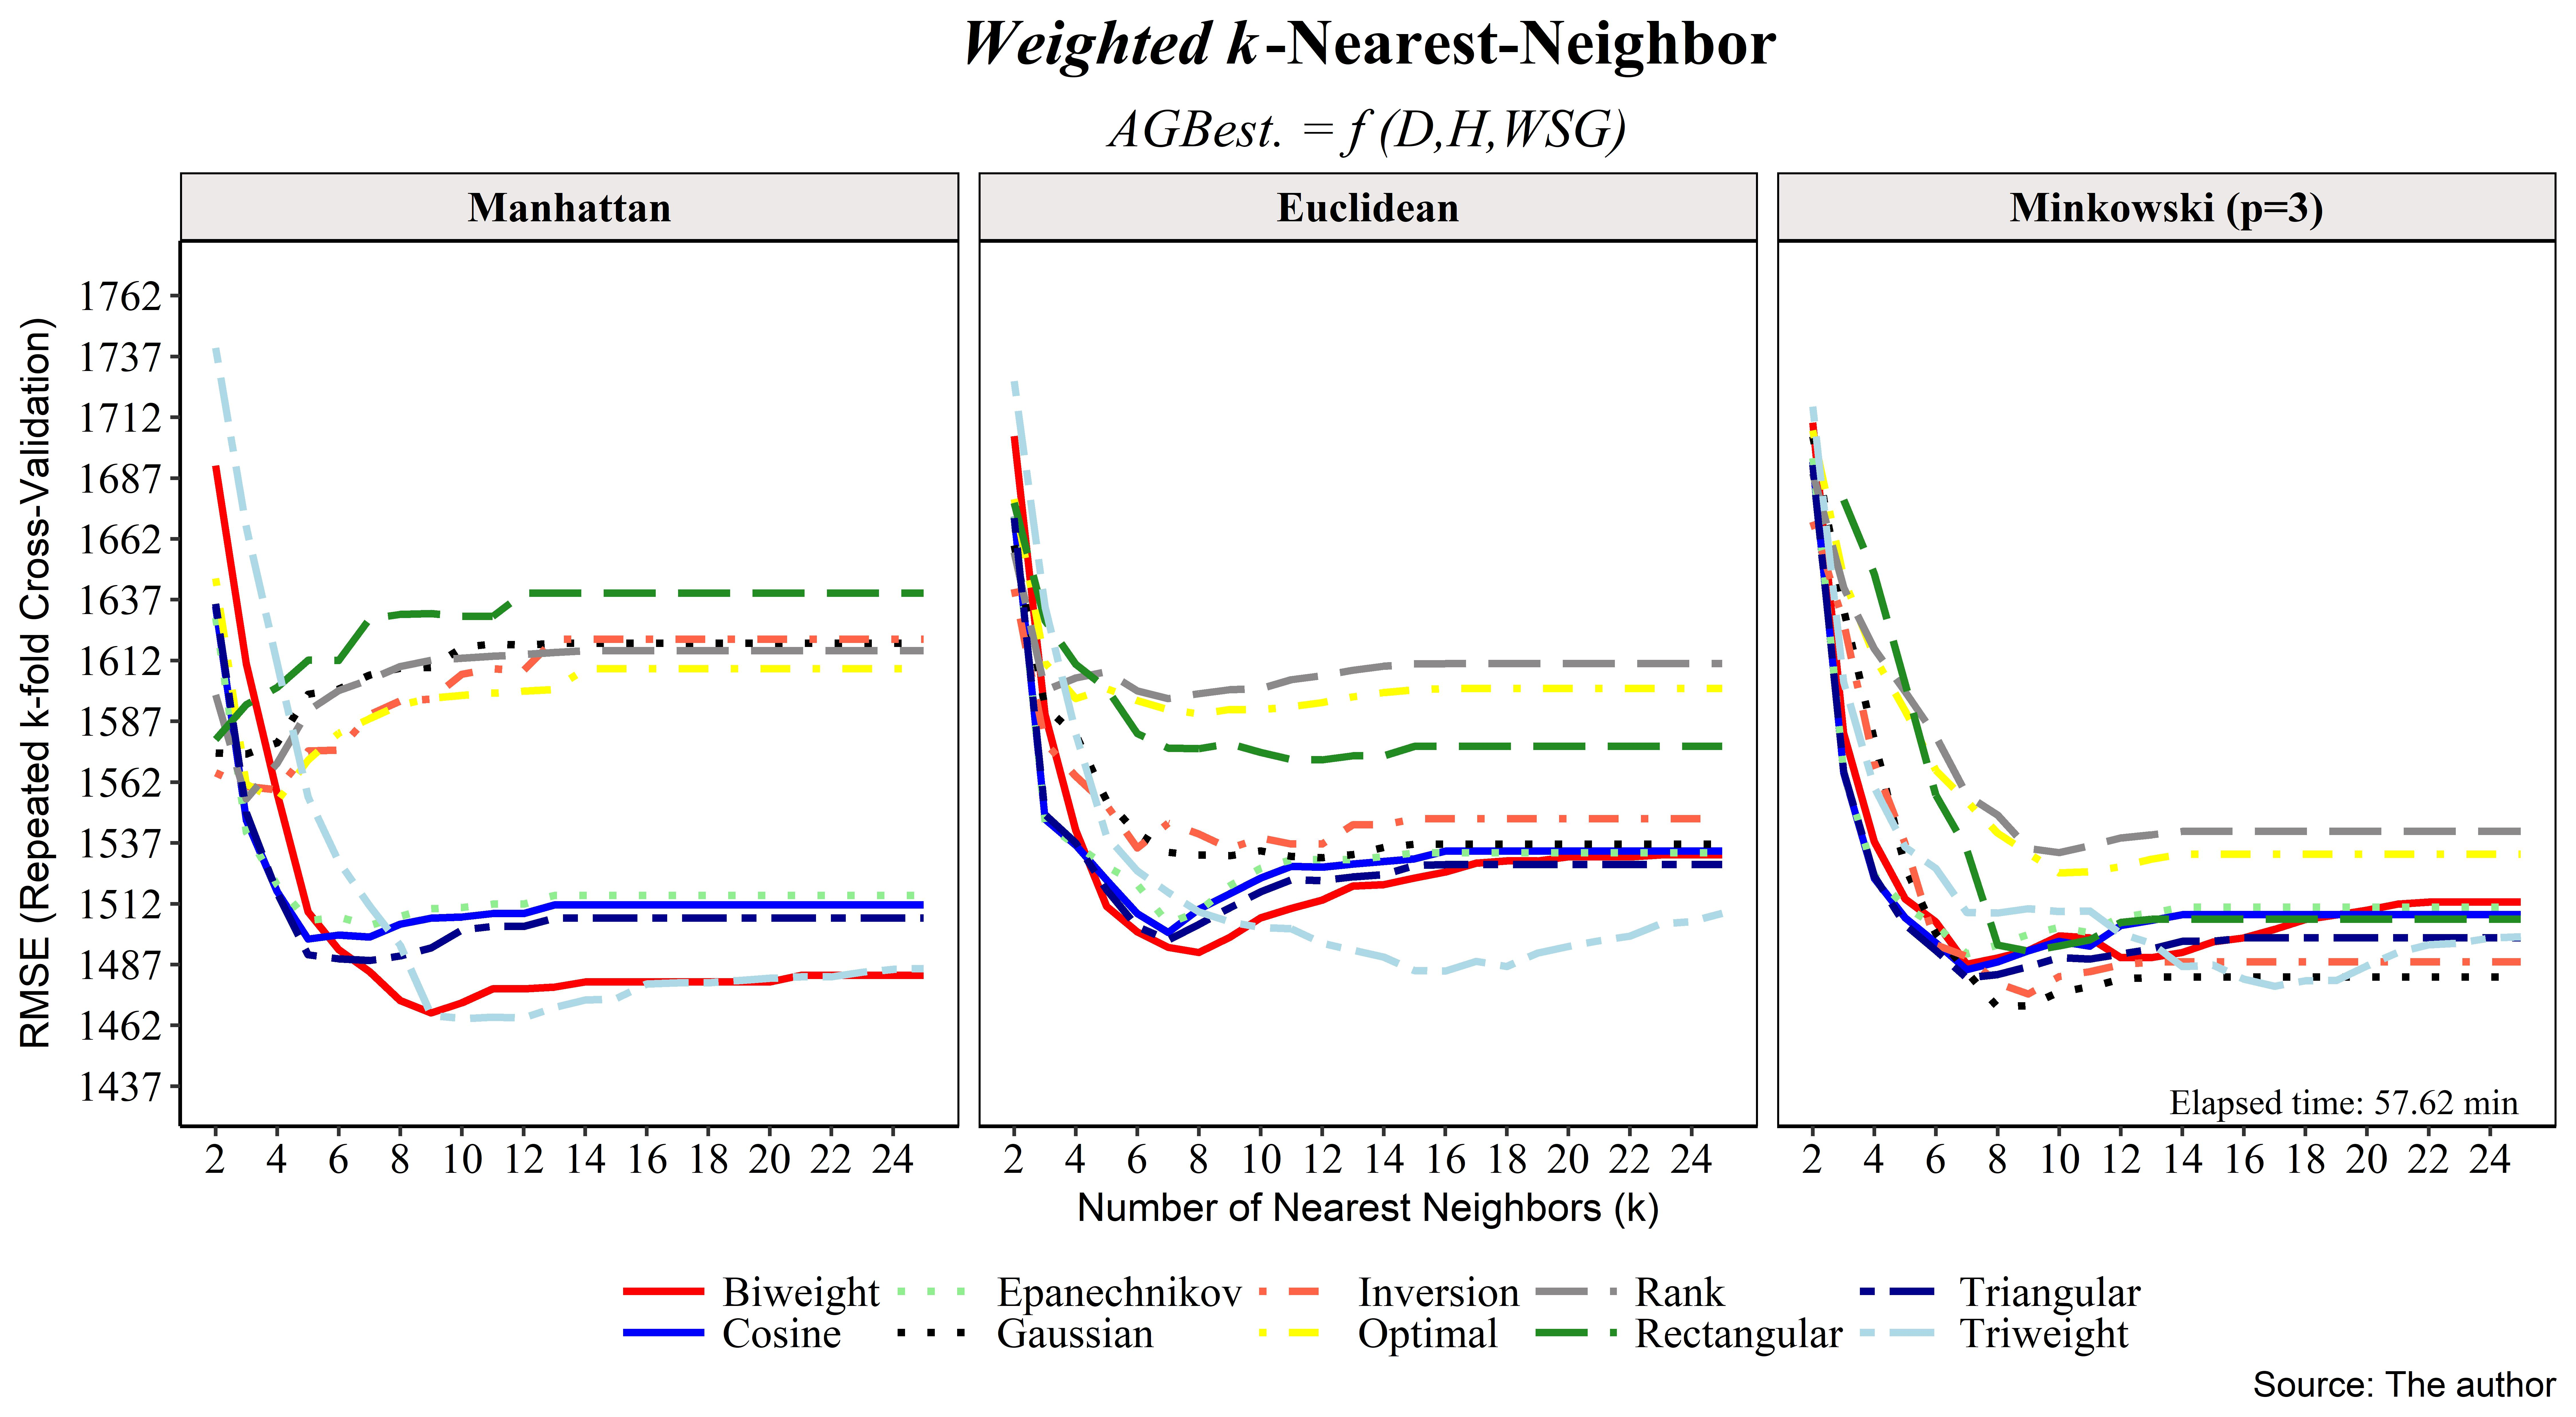
\includegraphics[scale=0.5]{Fig/Figura4A1}
	\end{center}
	
\end{frame}

%%%%%%%%%%%%%%%%%%%%%%%%%%%%%%%%%%%%%%%%%%%%%%%%%%%%%%%%%%%%%%%%%%%%%%%%%%%%%%%%%%%%%%%%%%%%%%%%

\begin{frame}[c]{Resultados Parciais}
	
	\centering
	\textbf{Pantropical Model} \textit{versus} \textbf{Modelo 9trwg}
	
	\begin{center}
		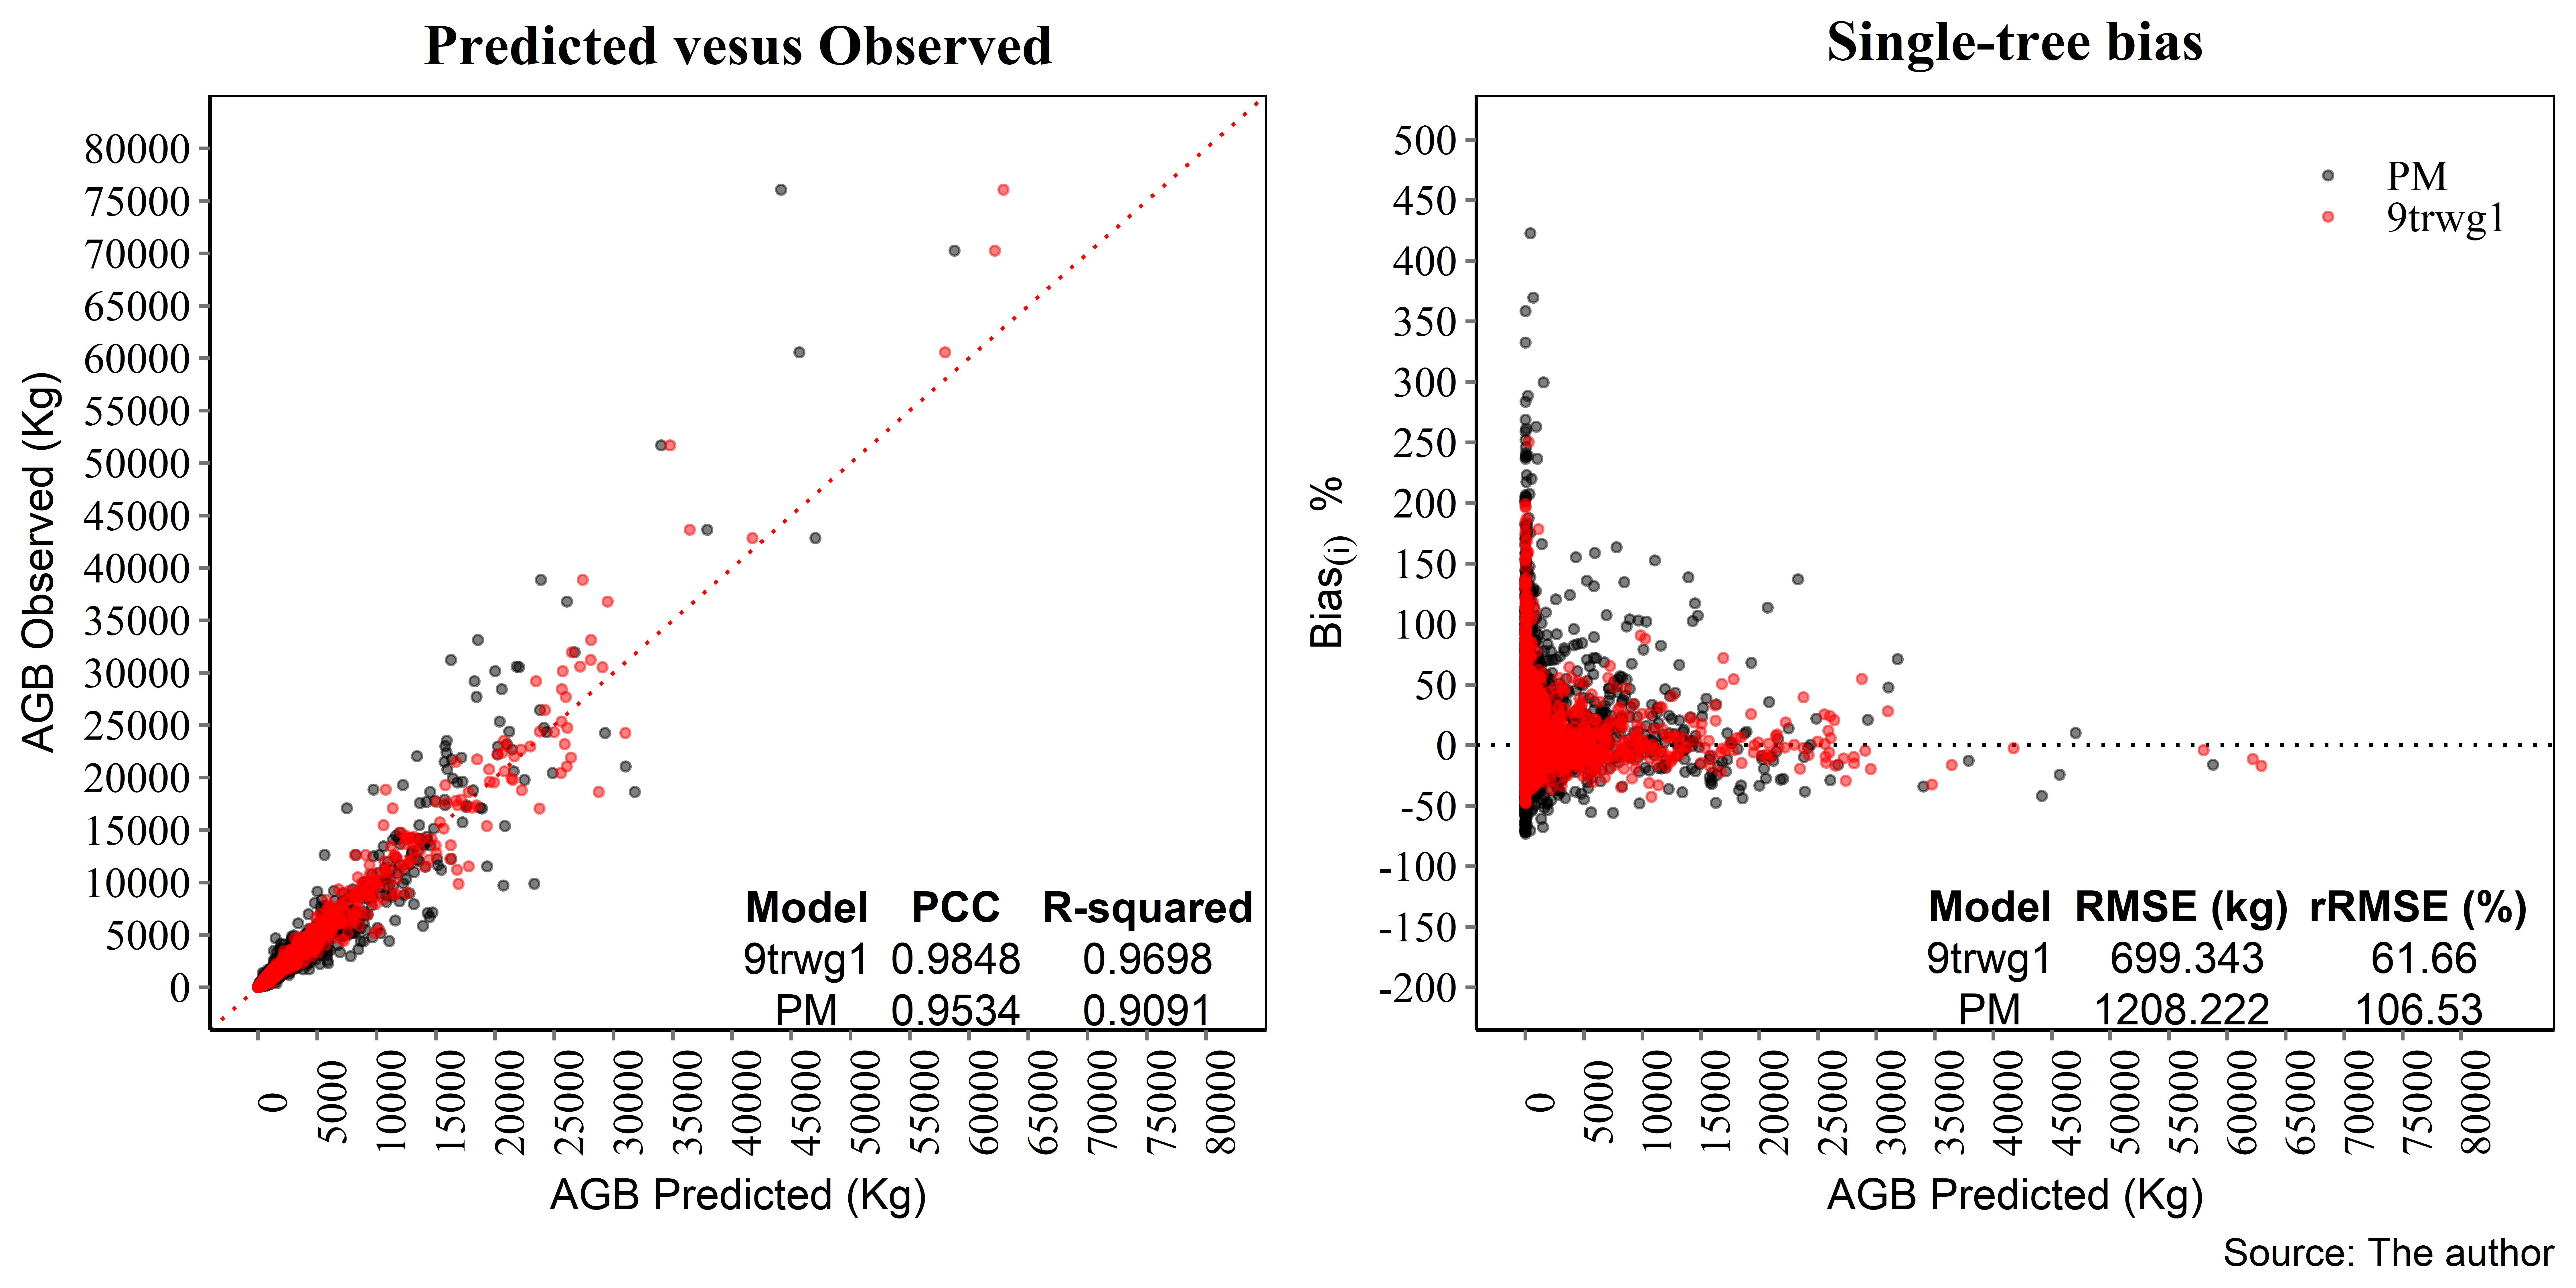
\includegraphics[scale=0.5]{Fig/CH_WkNN}
	\end{center}
	
\end{frame}

%%%%%%%%%%%%%%%%%%%%%%%%%%%%%%%%%%%%%%%%%%%%%%%%%%%%%%%%%%%%%%%%%%%%%%%%%%%%%%%%%%%%%%%%%%%%%%%%

\begin{frame}[c]{Resultados Parciais}
	
	\centering
	\textbf{Pantropical Model} \textit{versus} \textbf{Modelo 9trwg}
	
	\begin{center}
		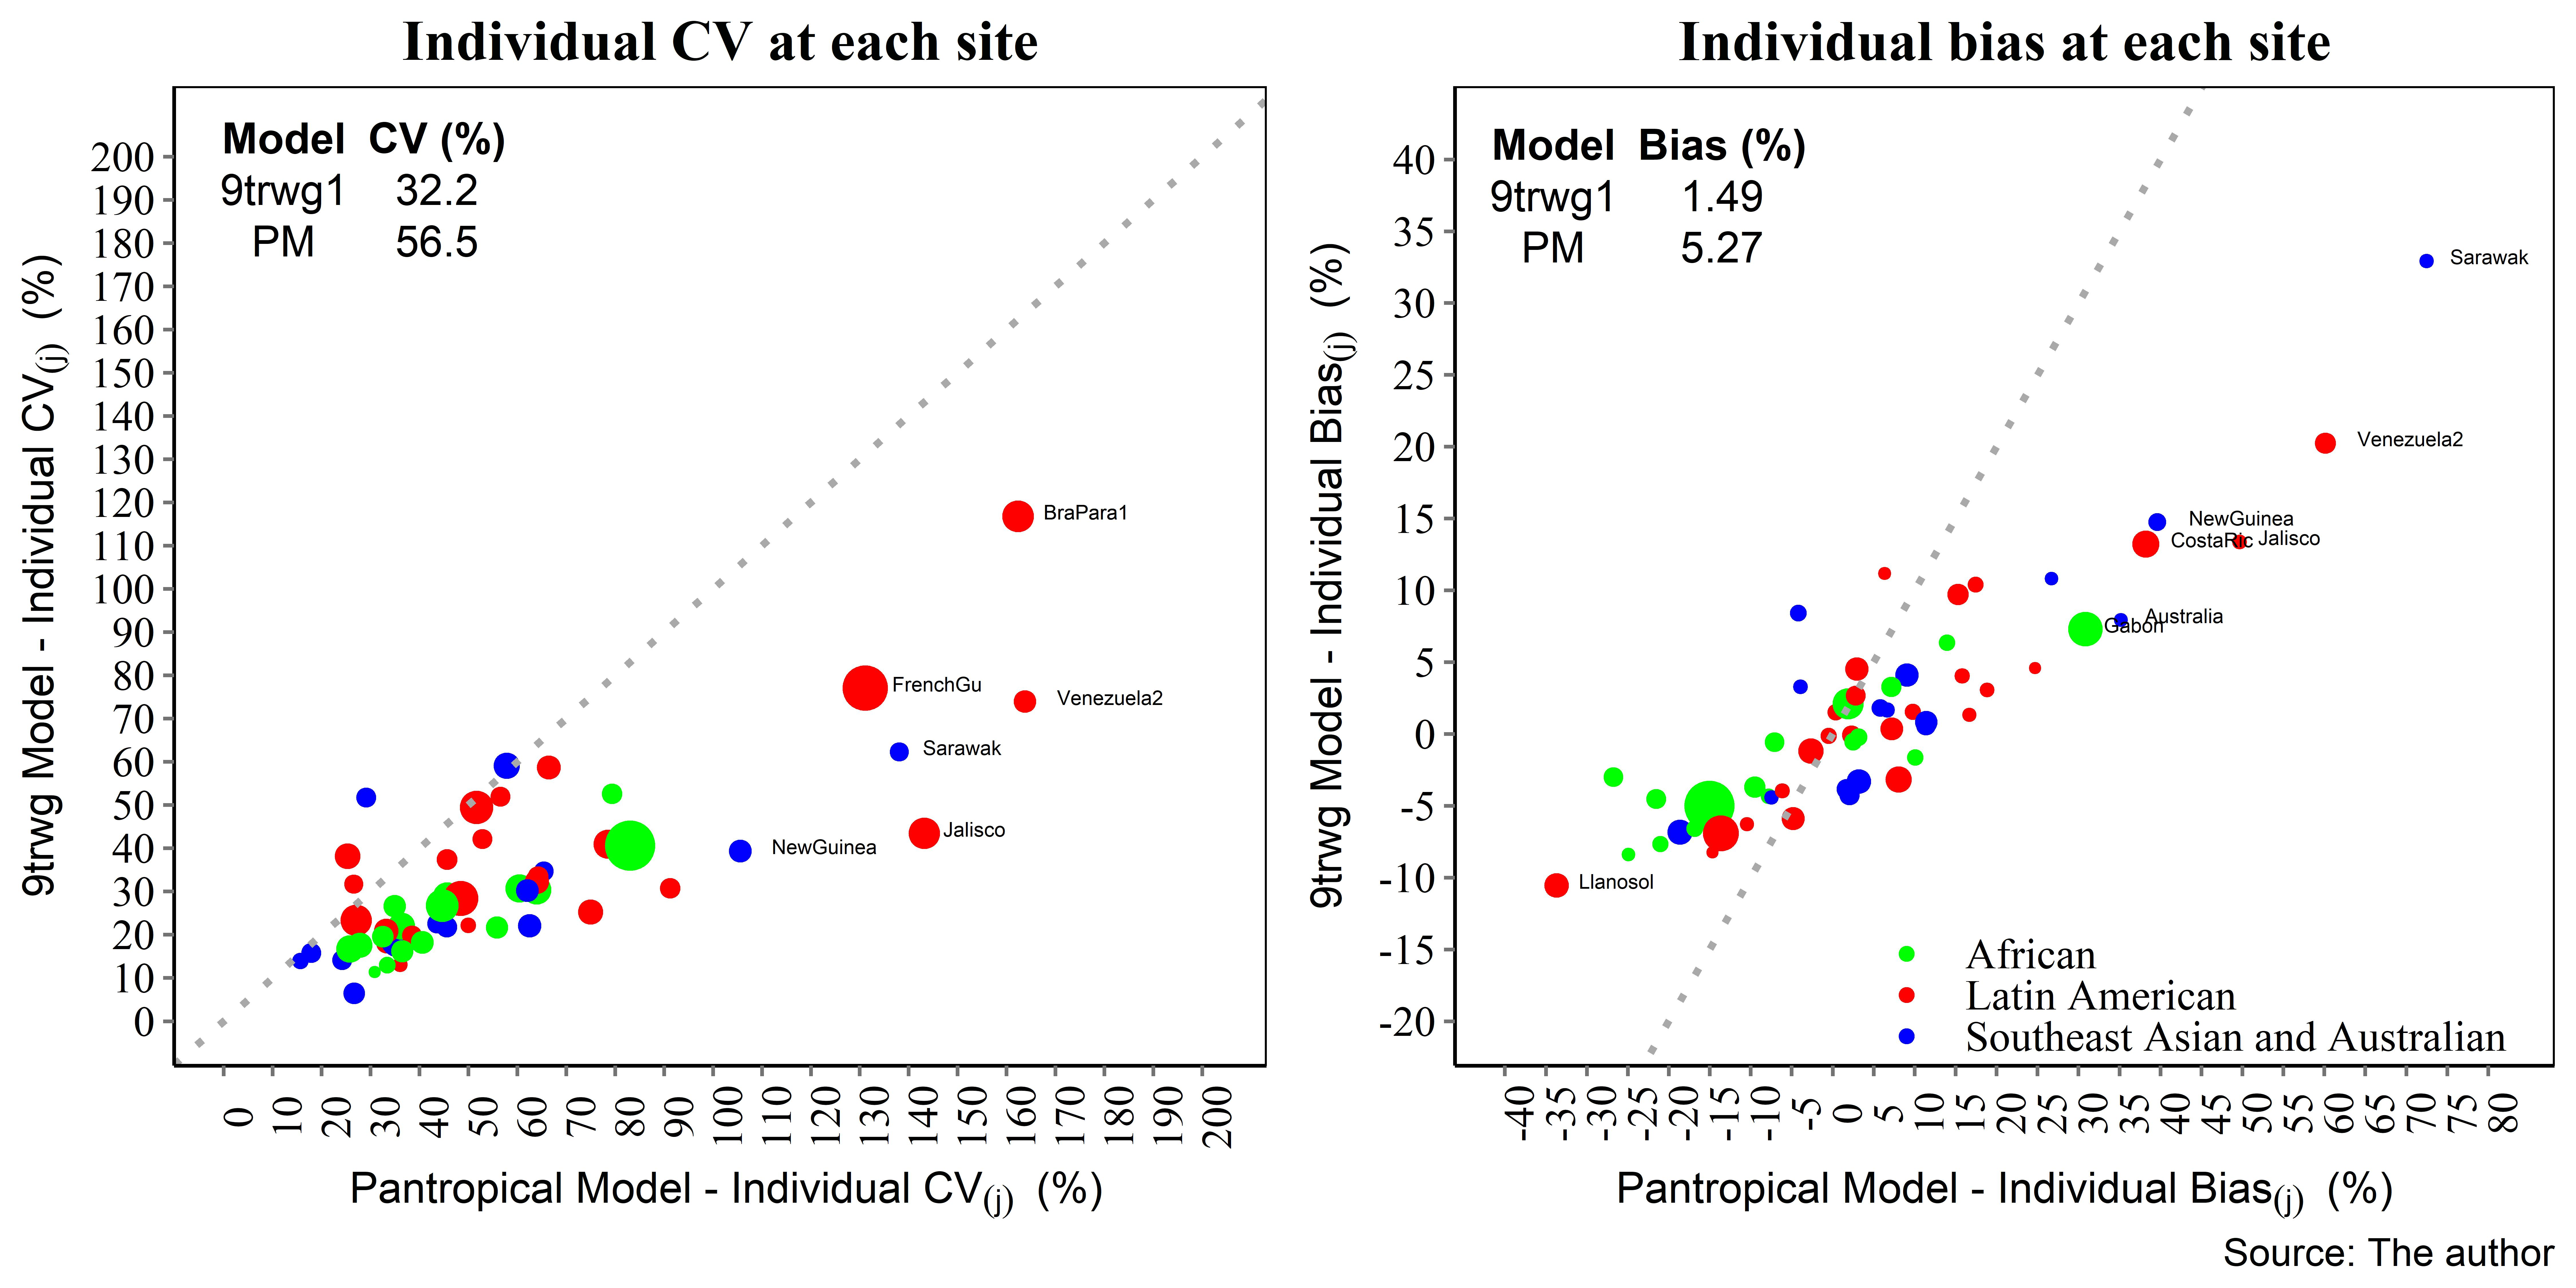
\includegraphics[scale=0.5]{Fig/CV_Bias}
	\end{center}
	
\end{frame}

%%%%%%%%%%%%%%%%%%%%%%%%%%%%%%%%%%%%%%%%%%%%%%%%%%%%%%%%%%%%%%%%%%%%%%%%%%%%%%%%%%%%%%%%%%%%%%%%
\begin{frame}[t]{Consideração Final}
	
	\textbf{CONSIDERAÇÃO FINAL} \newline
	
    \textbf{Estamos Entusiasmados! \dLaughey[2]} \newline
    
    \justifying
	\textbf{Avanço}: Precisamos compreender melhor e avançar na implementação de algoritmos de \textcolor{blue}{\textbf{Aprendizagem de Máquina}} para predição de variáveis nas Ciências Florestais! \newline \newline
	
	
	\Springtree[10]
	

\end{frame}
%%%%%%%%%%%%%%%%%%%%%%%%%%%%%%%%%%%%%%%%%%%%%%%%%%%%%%%%%%%%%%%%%%%%%%%%%%%%%%%%%%%%%%%%%%%%%%%%%
%BIBLIOGRAFIA
%%%%%%%%%%%%%%%%%%%%%%%%%%%%%%%%%%%%%%%%%%%%%%%%%%%%%%%%%%%%%%%%%%%%%%%%%%%%%%%%%%%%%%%%%%%%%%%%%
\begin{frame}[allowframebreaks]

	\textbf{Referencial teórico}
	
	\bibliography{refs}
	
\end{frame}

%%%%%%%%%%%%%%%%%%%%%%%%%%%%%%%%%%%%%%%%%%%%%%%%%%%%%%%%%%%%%%%%%%%%%%%%%%%%%%%%%%%%%%%%%%%%%%%%%
% AGRADECIMENTO
%%%%%%%%%%%%%%%%%%%%%%%%%%%%%%%%%%%%%%%%%%%%%%%%%%%%%%%%%%%%%%%%%%%%%%%%%%%%%%%%%%%%%%%%%%%%%%%%%
\begin{frame}[c]{}
	
	\begin{center}
		{\Large \textbf{OBRIGADO!}}
		
		Deivison Venicio Souza (UFPA) \\
		Programa de Pós-graduação em Engenharia Florestal - UFPR \\
		Email: deivisonvs@ufpa.br
	\end{center}
	
\end{frame}

\end{document}
